%
% File naaclhlt2010.tex
%
% Contact: nasmith@cs.cmu.edu

\documentclass[11pt,letterpaper]{article}
\usepackage{naaclhlt2010}
\usepackage{times}
\usepackage{latexsym}
\usepackage{amsmath}
\usepackage{tikz}
\usepackage{graphicx}
\setlength\titlebox{6.5cm}    % Expanding the titlebox


\title{Identification of Bacterial and Eukaryotic Genes using Interpolated Markov Model}

\author{Jacob Pritt\\
  {\tt mpritt4@jhu.edu}
  \And
  Guannan Ren \\
  {\tt gren3@jhu.edu}}

\date{}

\begin{document}
\maketitle
\begin{abstract}

\end{abstract}

\section{Introduction}
\paragraph{}
In the field of computational biology, gene identification and location is important in various applications such as controlling the expression level of genes. In the scope of the project, we seek to investigate a highly accurate gene identification tool which distinguishes coding and non-coding sections of the genome. We will also compare the IMM with fixed length Markov chains for the classification of coding regions. GLIMMER (Gene Locator and Interpolated Markov ModelER), is a tool designed to find the genes inside a microbial genome. It uses an interpolated Markov model which is an improvement upon the Markov chain model. In the original GLIMMER publication, the authors noted that from a test batch of hundreds of bacterial genomes, the software was able to achieve over 95\% accuracy on gene identification. For our project, we seek to implement the IMM algorithm used in GLIMMER and to match our classification results with that of the publication's. Next we will run our algorithm on eukaryotic genomes to examine the gene identification performances on eukaryotic species. We expect the accuracy of gene identification to drop significantly for eukaryotic genes, since eukaryotic genomes have highly complex coding sequences than that of the prokaryotes.\\

GLIMMER uses interpolated Markov models. IMMs are more powerful than simple Markov chains. A fixed-order Markov chain uses a fixed number of preceding bases to predict the DNA sequence. For example, a 5th order Markov chain would use five previous bases to predict the next base in the sequence. Markov chain run into problems when the training data is low such that the feature vectors created is too sparse to estimate the probability of bases after every combination of 5-mers. A kth-order Markov model would require up to $4^ (k+1)$ probabilities to be estimated from the training data. In order to estimate the probabilities, at least few occurrences of all possible k-mers must be present to yield a valid estimate. \\

It is often difficult for a training genome to have sufficient 5mers to provide a valid estimate. The interpolated Markov Model works around this problem by using a combination of probabilities of different length oligomers to give a better prediction. The IMM assigns different weights to each oligomer depending on its number of occurrences within the training DNA sequence. A highly frequent k-mer occurrence receives a higher weight while a low occurrence k-mer receives a lower one. When the sample data lacks a certain occurrences for a specific length oligomer, the IMM will resort to using a combination of the shorter oligomers sharing similar prefix sequence for its decision. 


\subsection{Reading Frame and Coding Sequence Description}

The original GLIMMER software first parts the DNA sequence into six different reading frames. Consecutive reading frames share the DNA sequence but differ on which nucleotide is first read. Since each nucleotide triplet specifies a codon during translation, there can be 3 different positions at which we can start reading codons at. And, three more reading frames applies to the reverse complement strand of the DNA. This gives us a total of 6 possible reading frame positions to find starting codons for coding sequences. 
From each reading frames, multiple open reading frames can be found. Each open reading frame is the DNA sequence that starts with the start codon and ends with the stop codon, without having any stop codon in the middle. However, there can be additional start codons in the reading frame. An ORF would generate a protein sequence once translated. 

\subsection{Why Identification of Coding Region Useful?}

Talk about the implication of matching the coding region with different gene expression

\section{Dataset Overview}

In our project, we seek to duplicate the results obtained from the original publication of GLIMMER. From the specifications of the original paper, we are using H. \emph{Influenzae} to test the IMM. The first 5000 DNA nucleotides within the complete H. \emph{Influenzae} genome are used to train our model, and the rest are used for testing. The complete genome for the organism was retrieved from GenBank database.

\section{Methods}
\subsection{Classification}

To better convey how the interpolated Markov model algorithm works, we will first explain how a Markov chain probabilistic model is able to classify its target. In a sense, a DNA sequence can be viewed as a sequence generated by a probabilistic model of the interactions between its random variables, which are the 4 coding nucleotides in our case. Each of the random variable can take the values of A, C, G, or T. The Markov chain probabilistic model captures this probability by enumerating the probabilities as states. The probability of a DNA nucleotide to take on a certain base depends on its previous neighbor in the DNA sequence. This can illustrated by observing the model for a simple 1-mer model as follows, \\
\begin{equation*}
P(S_{x+1} \mid S_{1}, .. ,S_{x}) = P(S_{x+1} \mid S_{x})
\end{equation*}
\\
TODO get rid of
\begin{figure}[h]
	\begin{center}
		\begin{tikzpicture}[style=thick,scale=1] 
		\newcommand{\nsize}{1.2}
		\begin{scope}[shape=circle,minimum size=0.5cm] 
		\tikzstyle{every node}=[draw,fill] 
		\node[fill=none,scale=\nsize] (State) at (0,0) {$\mathbf{State}$};
		\draw [->] (State) -- (State);
		\end{scope} 
		\end{tikzpicture}
		\caption{A directed graph}
		\label{fig:bn}
	\end{center}
\end{figure}

For a first order Markov chain, the occurrence probability of the nucleotide random variable $X_i$ only depends on the probability of the preceding variable $X_{i-1}$. This model can be extended to higher orders, in which the random variables will depend on additional preceding variables. For example, a k-th order Markov model specifies that $X_i$ will depend on variables $X_{i-k}$ to $X_{i-1}$. It is worth noting that by increasing the order of the Markov model, the predictive power of the model will steadily increase. However, by increasing the number of preceding variable probabilities, the space requirement for storing all of the combinations increases. For example, a first order Markov model will hold $4^2$ probabilities for nucleotide combinations, while a fifth order Markov model can potentially hold $4^6$ probabilities. \\

For a first order Markov chain, the current state of a variable is only dependent upon the previous state. We generalize this model to higher order by using addition states prior to predict the current state. The combination of Markov chains of different orders allows us to come up with the algorithm for an interpolated Markov model where the weights from different orders of Markov chain are tallied and used to produce a final score for the sequence. By choosing the model with the highest probability, we would figure out where the true coding region starts. \\

As mentioned, a higher-order Markov chain would do at least as well as a lower-order chain given sufficient training data. However, when we move to a higher-order Markov chain, the probabilities for sequences are sparse and the sparsity leads to inaccuracies. For rare k-mers not satisfying a certain occurrences threshold, the interpolated Markov model resorts to combining all probabilities from previous base sequences. There would be more data available for lower-order models since shorter sequences appear more frequently.


\begin{equation}
P(S \mid M) = \sum_{x=1}^{n} \mathbf{IMM_8}(S_x)
\end{equation}

\subsection{Features}
\label{ssec:layout}

\subsection{Feature extraction/selection}

We can compute the probability of base $s_x$ given the $i$ previous bases as

\subsection{Weight calculation}

In this section we describe how GLIMER computes the weights for the different kth-order IMM. First, a set of known coding sequences are assembled to a training set. To be certain these are truly coding is problematic at times. Hence, we decided to only use ORFs satisfying a certain nucleotide length requirements. \\
From the training set of genes, the frequencies of occurrences of all possible substring patterns of length 1 to k + 1 are counted and stored for each of the reading frames. If we consider a single reading frame at a time, and let $f(S)$ denote the number of occurrences of the sequence $S = s_1s_2..s_n$, then, we can get an initial estimates of the probability of base $s_x$ given the previous sequences $s_{x-i}, s_{x-i+1}, .. s_{x-1}$, which is denoted as $S_{x,i}$. The probability of base $s_x$ is given as the following:
\begin{equation}
P_i(S_x) = P(s_x \mid S_{x,i})  = \dfrac{f(S_{x,i})}{\sum_{be(acgt)}f(S_{x,i}, b)}
\end{equation}
The weight attached to $P_i(S_x)$ can be seen as a confidence measure of how close the estimated probability matches that of the true probability. GLIMMER computest the weight factor by first checking the frequency of occurrences for the k-mer sequence. When the frequency exceeds certain threshold value, the weight for the k-mer sequence is set to 1. However, the k-mer sequence frequency count is less than the threshold number, we resort to an alternate method for calculating the weight factor. (link to figure?). For a given context string $S_{x,i}$ of length i, we can compuare the observed frequenceis of all possible base pairings, $f(S_{x,i},a)$, $f(S_{x,i},c)$, $f(S_{x,i},g)$, and $f(S_{x,i},t)$ with the previously calculated IMM probabilities using the next shorter context, which is $IMM_{i-1}(S_{x,i-1},a)$, $IMM_{i-1}(S_{x,i-1},c)$, $IMM_{i-1}(S_{x,i-1},g)$, $IMM_{i-1}(S_{x,i-1},t)$. Now, using a $\chi^2$ test, we can determine how likely it is that the four observed frequences are consistent with the IMM values from the next shorter context. If the frequencies differ significantly from the IMM values, we would give them a higher weight since they would give us more information. The result of the $\chi^2$ confidence c can be used to designate a weight as follows:
\begin{equation}
\lambda_i(S_{x-1})=
\begin{cases}
0, & \text{if}\ c < 0.50 \\
\dfrac{c}{400}\sum_{be(acgt)}f(s_1,s_2..s_ib), & \text{if}\ c>= 0.50
\end{cases}
\end{equation}

For the purposes of reproducing the results of the research publication, we set our frequency of occurrences threshold to be 400. 
\begin{equation}
IMM_k(S_k) = \lambda_k(S_{k-1}) \cdot P_k(S_k) + [1 - \lambda_k(S_{x-1})] \cdot IMM_{k-1}(S_x)
\end{equation}


\section{Results}

As previously mentioned, we are using the complete H. influenzae genome to evaluate the performance of our IMM gene classifier. We ran the IMM algorithm under different training and test settings. We were able to evaluate the model performance at maximum k-mer length between the range 0 to 9. A maximum k-mer length of 0 indicates that we are predicting independently of the preceding nucleotide in the DNA sequence, while a maximum k-mer length of 9 indicates that the current nucleotide’s probability can be dependent upon at most 9 preceding DNA nucleotides. 

We implemented and tested fixed-length Markov chain models of orders between 0 and 9 to compare our IMM results against.

\subsection{Comparison of IMM and Markov chain on H.influenzae data}
Figure 2 shows how the IMM compares against the Markov chain model at identification of H. influenzae genes at the different model complexities.

When running our IMM and Markov chain programs, we imposed the same set of selection criteria as the mentioned in the publication. First, we would rule out all ORF’s that are less than 500 bases long, since longer ORF length are more likely to be coding regions. Next, we impose the constraint that the potential ORFs selected must not overlap one another. 

\begin{figure}
	\begin{center}
		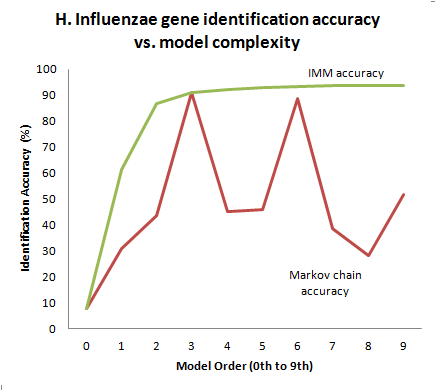
\includegraphics[scale=0.8]{plots/accuracy_vs_model_complexity.png}
	\end{center}
	\caption{\label{font-table} Accuracy comparison for IMM and MC models at different model complexity for \emph{H. influenzae} genome}
\end{figure}

Besides comparing the gene identification accuracies between our models, we chose to record the running time for our models as well. We ran both the IMM and the Markov chain models at different complexities on the H. influenzae genome to generate Figure 3. 

\begin{figure}
	\begin{center}
		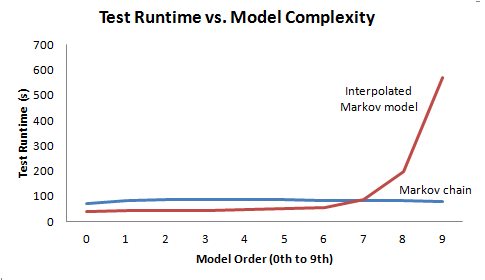
\includegraphics[scale=0.8]{plots/runtime_vs_model_complexity.png}
	\end{center}
	\caption{\label{font-table} Runtime comparison for IMM and MC models at different model complexity}
\end{figure}

We thought checking the number of false positives would be interesting. Figure 4 shows the counts of false positives selected by our models. 

\begin{figure}
	\begin{center}
		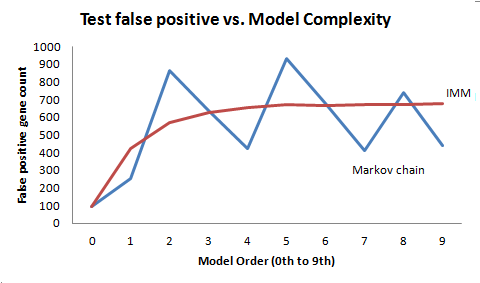
\includegraphics[scale=0.8]{plots/false_positives_vs_model_complexity.png}
	\end{center}
	\caption{\label{font-table} False positive gene identified for IMM and MC models at different model complexity}
\end{figure}

We were interested to see how our model generalize to other bacterial genomes, so we ran similar tests on H. pylori and E.coli genomes. The comparisons between an $8^th$ order interpolated Markov model and an $8^th$ order Markov chain for different prokaryotes are shown in Table 1.

\begin{table}
	\begin{center}
		\begin{tabular}{|c|c|c|}
			\hline \bf Organism & \bf MC Acc.(\%) & \bf IMM Acc.(\%) \\ \hline
			H. influenzae & 51.87 & 93.87 \\
			\hline
			H. pylori & 44.47 & 96.88 \\
			\hline
			E. coli & 27.92 & 58.79 \\
			\hline
		\end{tabular}
	\end{center}
	\caption{\label{font-table} Generalization of Markov chain and interpolated Markov model to other prokaryotic genomes at $9^{th}$ order complexity}
\end{table}


\subsection{Gene finding on Eukaryotic organisms}

While not mentioned in the original GLIMMER publication, gene identification on Eukaryotic genome sequences using the IMM is something we set out to test. Using the complete genome for Drosophila melanogaster’s chromosome X, we ran our IMM and fixed-length Markov chain algorithms to yield the results as shown in Figure 5.

\begin{figure}
	\begin{center}
		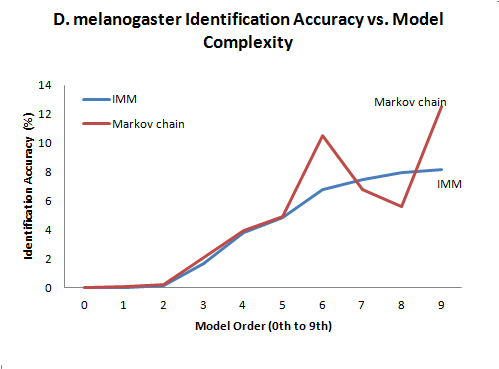
\includegraphics[scale=0.8]{plots/accuracy_vs_model_complexity_drosophila.png}
	\end{center}
	\caption{\label{font-table} Accuracy comparison for IMM and MC models at different model complexity for \emph{D. melanogaster} genome}
\end{figure}

We noticed the poor gene identification accuracy. This result is expected, since Eukaryotic genomes are much more complex than that of Prokaryote’s. For example, the extra non-coding intron sequences and the regulatory sequences such as promoters and enhancers increase the noise which our gene identifier has to go through. 

\subsection{Gene finding on with interpolated Hidden Markov Models}


\begin{figure}
	\begin{center}
		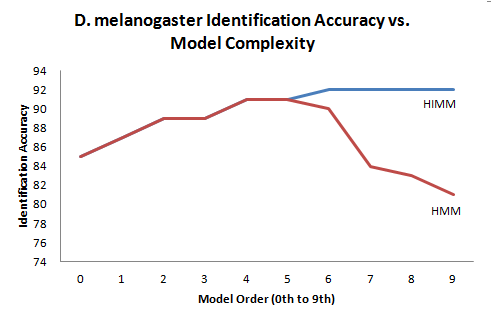
\includegraphics[scale=0.8]{plots/accuracy_vs_model_complexity_drosophila_hmm.png}
	\end{center}
	\caption{\label{font-table} Accuracy comparison for HIMM and HMM models at different model complexity for \emph{D. melanogaster} genome}
\end{figure}


\section{Discussion}

When comparing our 8th order IMM results against the same model as used in the publication, we notice that our accuracy value, of 93.78 \%, differs from the accuracy of 97.8 \% reported. There are several reasons that might have caused this difference.

We noticed there were 1717 annotated genes for the publication while our annotated gene file only contained 1174 genes. We suspect that they had additional experimental data to work with. This difference in the number of annotated genes only affected the number of false positive ORF turn outs in our results. Since we are mainly focused on replicating the results for true positives, we decided to ignore this difference.

From the fixed-length Markov chain results, we noticed that the identification accuracy peaks at intervals of three bases. We think that this might be due to the codon length. 

Overall, we are satisfied with the sensitivity of our IMM on the identification of true bacterial genes.

\subsection{Comparison to Project Proposal}
Judging by our original project proposal, we have accomplished the must-achieve milestones by implementing an IMM classification program closely following the program specifications of the GLIMMER publication. We have also managed to finish the features mentioned in the expected to achieve section. We have written a Markov model to compare the results obtained to that of the IMM’s. If we had additional time, we would likely to have accomplished the reach-goals for improving upon the IMM’s accuracy by training additional model organisms and to implement an interpolated context model to decide which positions to use for prediction.


\begin{thebibliography}{}

\bibitem[\protect\citename{Salzberg, S.L., Delcher, A.L., Kasif, S. and White, O.}1998]{Salzberg:98}
Salzberg, S.L., Delcher, A.L., Kasif, S. and White, O.
\newblock 1998.
\newblock {\em Microbial gene identification using interpolated Markov models}
\newblock Nucleic Acids Research: Oxford University Press.

\end{thebibliography}

\end{document}
